%% The '3p' and 'times' class options of elsarticle are used for Elsevier CRC
%% The 'procedia' option causes ecrc to approximate to the Word template
\documentclass[3p,twocolumn,times,procedia]{elsarticle}
%\documentclass[a4paper,10pt,twocolumn,preprint]{elsarticle}
%\documentclass[3p,times,procedia]{elsarticle}
\flushbottom

%% The `ecrc' package must be called to make the CRC functionality available
\usepackage{ecrc}
%% set the volume if you know. Otherwise `00'
\volume{00}

%% set the starting page if not 1
\firstpage{1}

%% Give the name of the journal
\journalname{Procedia Manufacturing}

%% Give the author list to appear in the running head
%% Example \runauth{C.V. Radhakrishnan et al.}
\runauth{H.S. Bank et al.}

%% Give the abbreviation of the Journal.
\jid{Protcy}

%% Give a short journal name for the dummy logo (if needed)
%\jnltitlelogo{Procedia Technology}

%% Hereafter the template follows `elsarticle'.
%% For more details see the existing template files elsarticle-template-harv.tex and elsarticle-template-num.tex.

%% Elsevier CRC generally uses a numbered reference style
%% For this, the conventions of elsarticle-template-num.tex should be followed (included below)
%% If using BibTeX, use the style file elsarticle-num.bst

%% End of ecrc-specific commands
%%%%%%%%%%%%%%%%%%%%%%%%%%%%%%%%%%%%%%%%%%%%%%%%%%%%%%%%%%%%%%%%%%%%%%%%%%
%% The amssymb package provides various useful mathematical symbols
\newcommand{\quotes}[1]{``#1''}
\usepackage{amssymb}
%% The amsthm package provides extended theorem environments
%% \usepackage{amsthm}

%% The lineno packages adds line numbers. Start line numbering with
%% \begin{linenumbers}, end it with \end{linenumbers}. Or switch it on
%% for the whole article with \linenumbers after \end{frontmatter}.
%% \usepackage{lineno}

%% natbib.sty is loaded by default. However, natbib options can be
%% provided with \biboptions{...} command. Following options are
%% valid:

%%   round  -  round parentheses are used (default)
%%   square -  square brackets are used   [option]
%%   curly  -  curly braces are used      {option}
%%   angle  -  angle brackets are used    <option>
%%   semicolon  -  multiple citations separated by semi-colon
%%   colon  - same as semicolon, an earlier confusion
%%   comma  -  separated by comma
%%   numbers-  selects numerical citations
%%   super  -  numerical citations as superscripts
%%   sort   -  sorts multiple citations according to order in ref. list
%%   sort&compress   -  like sort, but also compresses numerical citations
%%   compress - compresses without sorting
%%
\biboptions{sort&compress}

% \biboptions{}
% if you have landscape tables
\usepackage[figuresright]{rotating}
\usepackage{listings}

\begin{document}

\begin{frontmatter}

\dochead{46th SME North American Manufacturing Research Conference, NAMRC 46, Texas, USA}

\title{Temporal Logic (TL)-Based Autonomy for\\ Smart Manufacturing Systems}

\author[a]{Hasan Sinan Bank\corref{cor1}}
\author[b]{Sandeep D'souza}
\author[c]{Aditya Rasam}

\address[a]{Siemens Corporation, Corporate Technology, Princeton, USA} %755 College Road East, Princeton 08540, USA}
\address[b]{Carnegie Mellon University, Pittsburgh, USA}%5000 Forbes Ave, Pittsburgh 15213, USA}
\address[c]{North Carolina State University, Raleigh, USA} %27695, USA}

\begin{abstract}
%% Text of abstract
Smart-Manufacturing systems are increasingly being used to perform complex tasks on the factory floor. Most often, these systems have hard-coded cases to achieve a specific set of actions -or to assure the safety of the operations. The hard-coding makes the use complicated to re-deploy a system for different tasks. Therefore, it is necessary to have a flexible framework, which can generate a plan based on an intuitive description with system constraints, while satisfying all safety conditions. In this work, we propose Linear Temporal Logic (LTL)-based autonomy framework for smart-manufacturing systems. Specifically, we describe a general technique for formulating problems using LTL specifications. The use of LTL enables us to specify a manufacturing scenario (e.g. assembly), along with system constraints, as well as assured autonomy. Based on the given LTL formulation, a safe solution satisfying all constraints can be generated using a satisfiability solver. To eliminate the exhaustive and exponential nature of the solver, we reduced the exploration space with a divide and conquer approach in a receding horizon, which brings dramatic improvements in time and enables our solution for real-world applications. Our experimental evaluations indicated that our solution scales linearly as the problem complexity increases. We showcased the feasibility of our approach by integrating TL-based autonomy with the simulations of Gantry robot in Siemens NX Mechatronics Concept Designer and TIA Portal (PLCSIM Advanced) for Siemens S7-1500 TCPU connected to Sinamics drives. 
\end{abstract}

\begin{keyword}
autonomous cyber-physical systems; linear temporal logic; intelligent manufacturing systems; task planning; safe assured autonomy

\end{keyword}
\cortext[cor1]{Hasan Sinan Bank. Tel.: +1-609-734-6500}
\end{frontmatter}
\email{hasan.bank@siemens.com\vspace*{-25pt}}

\vspace*{-10pt}
\section{Introduction}
\label{main}
Manufacturing is an activity centered around the idea of converting raw-materials or partially-finished assemblies, into value-added products. To make profits, it is essential that the manufacturing process be flexible and cost-effective. A number of manufacturing inputs, such as the cost of raw materials and labor, are subject to internal and external perturbations which are influenced by innovation, public policy, and the state of the environment as well as the economy. To adapt those \newpage\vspace*{10pt}changes and reduce the total cost of manufacturing, researchers in industry and academia push the limits of the technologies in several topics including automation and robotics.Most of these technologies involve bridging concepts from multiple domains to build frameworks such as Industry 4.0 which incorporate several important factors such as autonomy, digital-twin and simulation \cite{digit_twin}, networking and connectivity \cite{smart_man}, cyber security \cite{cyber_sec}, cloud and edge computation \cite{hotcloud}, data analytics, and big data \cite{cloud_manuf}. The main aim of using these technologies is to build smart and versatile manufacturing systems, which can perform a variety of different tasks.

Synthesizing controllers for assured safety of autonomous cyber-physical systems is a necessity for systems operating on the factory floor because (i) humans and robots may perform collaborative manufacturing tasks, and (ii) violating safety requirements may cause damage to manufacturing equipment, raw materials or the environment. In addition to safety, the methodology for enabling autonomy should connect the previously highlighted aspects of Industry 4.0. 

Irrespective of the target industry or application, autonomous cyber-physical systems utilize intelligent algorithms for performing specific tasks without human intervention. Intelligent algorithms often incorporate meta-operating systems (e.g., ROS \cite{ros_item}) with both high and low-level controllers, which consist of closed-loop mechanisms for maintaining continuous stability, with respect to given decisions or planning results under constraints.

Several tests are required to conform and ensure the behavior of the system for the expected outputs. In most complex systems, it would be an exhaustive and almost impossible to cover all of the possibilities. Therefore, there are methods in software engineering such as model checking, to determine if the system model conforms to a given set of desirable properties. Model checking tools verify the functionality of a program structure in a concurrent event-driven fashion -similar to the operation flow of the factory floor. Nonetheless, it is notoriously difficult to validate all the reactions to non-deterministic interactions. To cope with these difficulties, we propose a methodology -commonly known as temporal logic (TL) specifications- which can be easily combined with the hardware- or software-in-the-loop systems for cyber-physical systems. Instead of programming the individual corner-cases in an in-depth finite-state specifics, we define the temporal-logic-based expressions with an intuitive input language specified in NuSMV solver \cite{nusmv2}. Our approach eases the implementation by using a mathematical formalism of logical operations with temporal specifications which enable smart manufacturing on factory floor.

From a software verification perspective, LTL is also advantageous to ensure safe operation of safety-critical systems. Other than software verification,one can give several examples of the applications from academia with different intentions such as prognostics and health management \cite{ltl_phm}, model-checking based verification approach for advanced industrial automation solution \cite{ltl_mod}, formal verification and code reuse for PLC-based automation systems \cite{ltl_plc}, formal specification language for control logic \cite{ltl_formal}, and symbolic planning tool to control robot motion \cite{ltl_control}. 
Most of these research efforts in academia and industry target a specific and tailored need to use TL in smart cyber-physical systems without having the generalization in a framework. Differently, the contributions of this paper are as follows:
\begin{enumerate}
\item Eliminating large and hand-coded formulations by using Linear-Temporal-Logic-based problem representations.
\item Reduction in the exploration space and ensuring the scalability of the approach within an acceptable runtime requirements.
\item Connectivity to a generic run-time framework for autonomous factory operations.
\item Integrating realizable, tractable, and satisfiable safe meta planner to an autonomous run-time framework.
\end{enumerate}

The rest of the paper is organized as follows. Section 2  provides insights into how Linear Temporal Logic (LTL) can be used for autonomy in smart-manufacturing systems. Section 3  showcases an example use-case of the proposed approach, in an autonomous industrial-automation laboratory setup, which contains an intelligent machine structure -Gantry Robot- for utilizing our proposed formalisms. Section 4 presents experimental results, and Section 5 concludes the paper.
\vspace{-10pt}
\section{Linear Temporal Logic (LTL)-based Autonomy for Manufacturing} \label{sec:ltl-autonomy}
Linear Temporal Logic \cite{LTL}, also known as LTL, is a mathematical description language, used to specify the behavior of a system over discrete time steps. Using LTL, a formula describing a set of paths consisting of different state transitions can be specified. For example, LTL can be used to specify a condition which will eventually be true, or a condition which holds until a specified state is reached. LTL was initially designed as a framework for specifying the properties of computer programs. Based on the specified set of properties, a program can be formally verified. In recent years, LTL has been increasingly used to specify planning problems \cite{ltl-planning}. The problem specification is generally the final state or goal to be achieved, while the constraints can include both the physical constraints, the model describing the system, as well as safety requirements. A satisfiability solver can then be used to generate a feasible solution path which can solve the specified problem, while satisfying the constraints. %, in a near-optimal fashion. 
Thus, the use of LTL enables a solution which satisfies all safety constraints, thus ensuring that a generated solution can provide safe autonomy.

We now briefly describe the semantics of LTL, in the context of specifying a manufacturing task.  Every LTL formula consists of a set of atomic propositions ($AP$) and several boolean and temporal operators. The following grammar is used to form LTL formulas \cite{model-book}: $\varphi$ ::= true $|$ a $|$ $\varphi_1$ $\wedge$ $\varphi_2$ $|$ $\neg$$\varphi$ $|$ $\bigcirc$ $\varphi$ $|$ $\varphi_1$ $\cup$ $\varphi_2$, where $a$ $\in$ $AP$ and $\bigcirc$ (next, i.e, $\varphi$ is true in the next time step), $\cup$ (until, i.e, some property holds until $\varphi$ is true). Other useful temporal operators include, $\square$  (always, i.e, $\varphi$ is always true), $\blacklozenge$ (eventually, i.e, $\varphi$ is eventually true) and $\Rightarrow$ (implication, i.e, $\varphi_i \Rightarrow \varphi_j$ implies if property $\varphi_i$ is true, then property $\varphi_j$ holds as well). A more detailed description of LTL can be found in \cite{model-book}.
%and refer the interested readers to Chapter 5 of [1] for details. 

Atomic Propositions ($AP$) are generally used to describe the properties of interest about a system. In particular, using multiple such propositions we can capture complex behavioral rules, system constraints and the planning objective. %LTL is particularly useful to generate complex behaviors given some general instructions and rules of the mission. 
Consider a typical automated manufacturing scenario involving the assembly or the additive construction of a certain object. This use-case generally involves the motion of one or more robotic tools, to successfully assemble/construct the object. To do so, a meta-planner as well as a tool-path needs to be generated for each tool, such that:\vspace{-10pt}
\begin{enumerate}
\item The time and energy required to construct/assemble the object is minimized.
\item The physical constraints of the tool and the workplace are not violated.
\item No safety constraints are violated.
\end{enumerate}

Some of the common physical constraints are including and not limited to reachability constraints, i.e., the part of the workspace accessible by the tool, and collision constraints, i.e., no two objects (tools, workpiece and obstacles) can be in the same place at the same time, to name a few. %Common safety constraints may include ...
One can easily increase the number of rules by converting standardized and formal definitions (e.g., \cite{NIST}, \cite{ISO-15066}, \cite{ISO-10218}, etc.) into TL formalisms which we present with this paper. 

We now describe how LTL can be used for autonomy in the manufacturing context. We use LTL as a language to generate a high-level specification for a planning problem. Based on this specification and a finite-state machine model of the system, we can generate a feasible meta-level sequence of tasks, which can be fed to low-level motion controllers for generating trajectories for the various system actuators. 

Without loss of generality, let us consider an assembly task to be carried out by a single tool, $\tau$, whose state can be described by an $M$-dimensional array $\tau_i,$ $i=1,2,3,...,M$. Each $\tau_i$ can be used to describe different properties, including those related to the the orientation or state of the tool. For example, if the tool is a gripper, its state variables $\tau_i$ can include (i) whether the gripper is open or close, (ii) encode its orientation based on its degrees of freedom, or (iii) specify the content which the gripper is holding. 

Let us assume that we have a 3-dimensional workspace, which can be divided into $N$ unit-size cubes $\pi_i,$ $i=1,2,3,...,N$, where the unit size depends on the resolution of the tool's motion or the granularity of the task, and $N$ depends on the size of the workspace and the chosen unit size. At any discrete time step, the state of each cube depends on the object occupying the space described by the cube. For example, the state of the cube can be empty $\epsilon$, or occupied by a tool $\tau$, an obstacle $\omega$, or a sub-assembly or part $\alpha_j, j=1,2,3,...,K$ where $K$ is the number of parts. We can assume that the state space for each $\pi_i$ is $ \Gamma = \{\epsilon, \tau, \alpha_j, \omega\}$, i.e, $\pi_i \in \Gamma, \forall i=1,2,3,...,N$. If we consider an assembly problem, the final objective can be described using the different $\pi_i$s, where to successfully assemble an object, each sub-assembly or part $\alpha_j$ should go to the its corresponding desired location $\pi_i$. Let this final desired state be $\Pi = \bigwedge_{i,j} \pi_i = \alpha_j$. Similarly, let the constraints of the system be $X$, which can be specified using temporal and logical operators.

Given the different planning objective $\Pi$ and constraints $X$, the LTL specification $\Delta$ of the manufacturing planning problem can be given by:

\begin{equation}
\Delta = X \cup \Pi
\end{equation}

This formulation implies that we need to find a solution path which can reach the state $\Pi$, such that the path satisfies all the constraints encoded by $X$ \textit{until} state $\Pi$ is reached. Among all such feasible paths, we are often interested in the path which can reach the desired state $\Pi$ in the shortest number of steps. 

However, to find a feasible plan representing the system state transitions, we also need to represent the manufacturing system as a finite-state machine. In the context of the manufacturing problem, the system state transitions can be described using the state of the tool $\tau$ and the state of the workspace $\Pi$. Using these state variables we can define deterministic transitions or let a solver randomly pick a state. For example, in this work, we are primarily interested in finding a feasible plan for a particular tool. Therefore, the transition of the tool's state (like position and orientation), needs to be chosen by the solver. Therefore the transition definitions for the tool in the state-machine representation is not deterministic. On the other hand, the next state of the workspace depends on the next state of the tool. For example if a gripper tool moves a sub-assembly from one location to another, there needs to be a corresponding change in the state $\Pi$, to reflect this movement. In Section \ref{sec:use-case}, by means of an example we will describe how the finite-state machine representation can be formulated.

Given an LTL specification along with the finite-state machine representation of the manufacturing system, we can find a feasible plan which violates for the given specifications, using a Bounded Model Checker (BMC) \cite{nusmv2}. Therefore, for our manufacturing problem, we need to provide a negation of the LTL specification derived in Equation 1, i.e., $\neg \Delta$, to find a feasible solution using a BMC. Most available BMCs use a Boolean Satisfiability (SAT) solver to find the shortest path which violates the given LTL specifications. Therefore, if the LTL consists of multiple states, the solution space can explode, which can result in the solver taking a long duration of time to generate a solution. In this regard, BMC-based solver becomes unrealistic for generating solutions in real-time. In Section \ref{sec:use-case}, we will explore how the solving time can be reduced by breaking up the problem into smaller pieces, using a divide and conquer in a receding horizon.

\begin{figure*}[t!]\vspace*{4pt}
\centerline{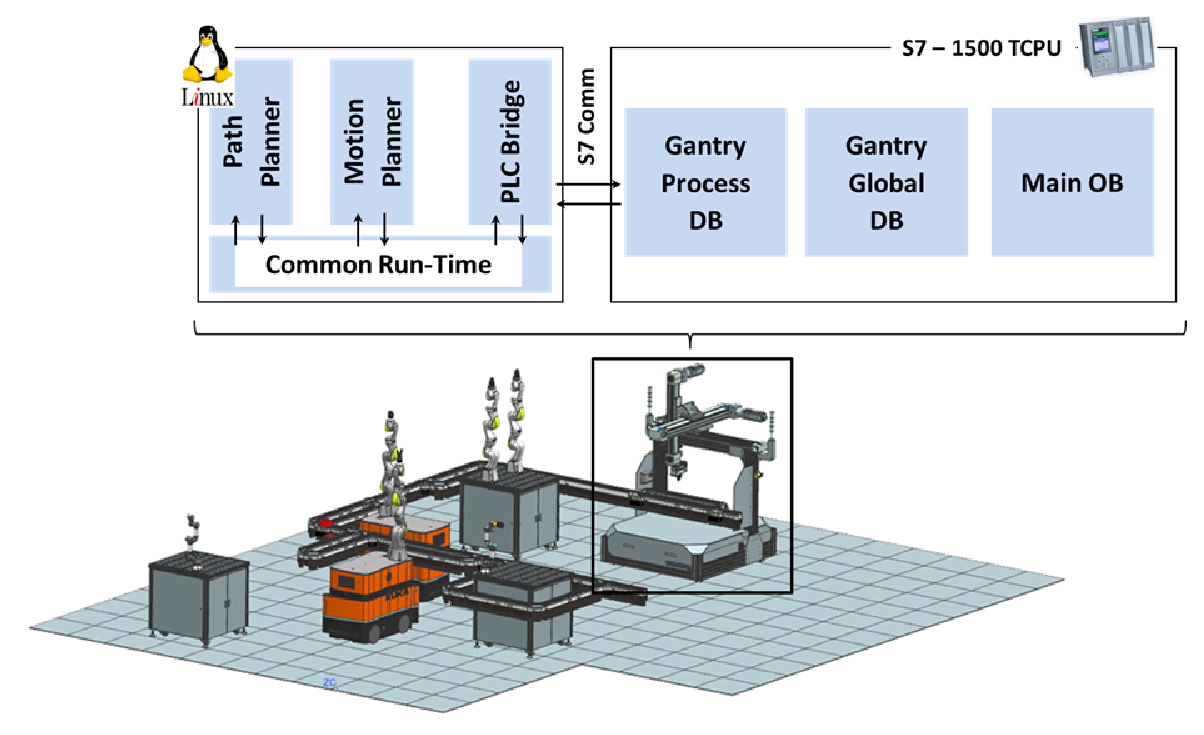
\includegraphics[width=150mm,scale=0.5]{figure1_}}
\caption{Application architecture for autonomous factory setup and intelligent machine tool (Gantry Robot in black rectangle)}
\end{figure*}
\vspace*{-10pt}
\section{Industrial Smart Manufacturing Test Bed} \label{sec:use-case}
In this section, we describe the industrial test-bed used to prototype our LTL-based task-planning methodology for smart manufacturing systems. Our system consists of gantry station, different type of industrial robot arms as well as smart conveyor system -as shown in Fig.1. We used gantry robot as an inspection and final assembly station to make sure the conformity between the target and current assembly. The robot arms performs intermediate operations before final assembly at the gantry robot. Smart conveyor system moves the products from one station to another. Our smart manufacturing test-bed represents a mission-driven production where the product carries the results in between object engines. For example, the product object can convey the perception from the sensors (e.g., cameras) to corresponding algorithms (e.g., station scheduler and planner) so that the smart conveyor is able to carry the product accordingly. Before going into the details of the design for our gantry robot, we describe a prototype use-case, for emulating a manufacturing scenario without the overall planning and scheduling between the stations.
\subsection{Autonomy Prototype Use-Case}
Our use-case imitates the assembly of multiple components by means of a \textit{puzzle}, which we provide to our Gantry Robot to \textit{solve}. The puzzle consists of a $A\times B$ 2-dimensional grid, with each space in the grid being able to accommodate a single colored cube. Initially all but one of the spaces in the grid are filled with cubes of $C$ different colors, where $C \leq (A\times B) -1$. Using a Human-Machine Interfaces (e.g. HMI touchpad, augmented reality, etc.), a user can specify a final configuration of the cubes presenting on the grid. The objective of the gantry system is to autonomously move the cubes to their user-specified positions, using the single empty space on the grid as a buffer. To do so, we use the LTL-based meta task-planning methodology described in Section \ref{sec:ltl-autonomy}, to formulate the problem. 
In order to use the proposed methodology to generate a feasible plan and tool-path, we developed a software package which utilizes the Bounded Model Checker (BMC) of NuSMV solver \cite{nusmv2}. Our package takes in the initial state of the system (which may be obtained from a camera or manual input), along with the desired user-specified state (from the Human-Machine Interface e.g., HMI TP700), and generates a problem specification as well as state-machine representation of the system. Our solution feeds the generated problem representation to the NuSMV BMC, which generates a safe and feasible meta-level plan. The motion planner module in our solution, can use this meta-plan for the execution of the plan. All of these mentioned algorithmic components are imbued in the controller (Siemens S7 TCPU) of the Gantry system with an architectural relationship is shown at the top of Fig 1.
In our gantry system, the provided \textit{puzzle} consists of a $6\times 4$ grid ($A=6$ and $B=4$), and consists of 23 cubes of 5 colors: red, green, blue, white and yellow ($C=5$). One space in the grid is empty, and serves as a buffer to move the cubes around. To illustrate how our proposed methodology works, we provide a toy-example of a $2\times 2$ grid, consisting of 3 cubes colored red (r), blue (b) and green(r), and one empty buffer space. 
Listing \ref{lst:nusmv-rep} provides the state-machine representation of the $2\times 2$ puzzle, and the LTL specification of the problem, using a NuSMV-compatible syntax \cite{nusmv2}. The representation provides a state-machine description of the problem, where the position of the gripper tool (\texttt{tool\_pos}) can be in any one positions (0,1,2 or 3) in the 2D grid. This tool position needs to be generated by the solver. Based on the position chosen for the gripper, the rest of the system state-transitions can be defined. For instance, the representation assumes that when the gripper tool is at a position in the grid, and if the gripper or the position is empty (no cube present), then the gripper and the space interchange the cube. For example, if the gripper is empty, and in a position with a cube present, the gripper picks up the cube, and the space becomes empty. Similarly, if the gripper has a cube and is in an empty position, the gripper releases the cube into the empty space. Thus, using the above assumptions, the state of any position in the grid (\texttt{pos0,pos1,pos2,pos3}) and the state of the gripper tool (\texttt{t\_state}) can be defined, using a switch-case syntax, which depends on the chosen tool position (\texttt{t\_pos}). {\newline}
The representation in Listing \ref{lst:nusmv-rep} also includes the LTL specifications of the problem, formulated using the methodology in Section \ref{sec:ltl-autonomy}. The LTL specification states a system constraint $X$, which specifies that the tool (gripper) should not place a cube in a space which is already occupied by another cube. For each position in the grid, this constraint is stated in the form, if the tool is at a position, and the state of the gripper tool is not empty (the gripper has a cube), then this should imply that the position is empty (does not have a cube). The stated LTL specification also has the final desired state $\Pi$, which is a logical AND of the final user-desired state of each of the positions in the $2\times 2$ grid. Therefore, the LTL specification is $\Delta = X \cup \Pi$. Thus, the input to the BMC is $\neg \Delta$, as the BMC is generally designed to find a path which does not meet the given specification. Figure \ref{fig:example} illustrates the result of an feasible solution path, generated using our solver package, for moving between a given starting state and user-specified end state.
\begin{lstlisting}[caption={NuSMV-based Problem Representation},label={lst:nusmv-rep}]
MODULE main
# Define the State Variables
VAR
t_pos     : {0,1,2,3}; 
t_state	  : {r,g,b,0}; 
pos0      : {r,g,b,0}; 
pos1      : {r,g,b,0}; 
pos2      : {r,g,b,0}; 
pos3      : {r,g,b,0}; 
empty     : {0,1,2,3}; 

# Initializing the State Variables
ASSIGN
init(t_pos)  	:= 0; 
init(t_state)	:= 0; 
init(pos0)      := r; 
init(pos1)      := g; 
init(pos2)      := b; 
init(pos3)      := 0; 
init(empty)     := 3; 

# System State-Machine Representation

# Tool Position
next(t_pos)   := {0,1,2,3};

# Tool State
next(tool_state) := case
	t_pos=0   : pos0;
	t_pos=1   : pos1;
	t_pos=2   : pos2;
	t_pos=3   : pos3;
	TRUE         : arm_state;
esac;

# Next empty state 
next(empty)                      := case
	t_pos=0 & next(pos0)=0     : 0;
	t_pos=1 & next(pos1)=0     : 1;
	t_pos=2 & next(pos2)=0     : 2;
	t_pos=3 & next(pos3)=0     : 3;
	TRUE                       : empty;
esac;

# Next State of Position 0 
next(pos0) := case
	t_pos=0 : tool_state;
	TRUE       : pos0;
esac;

# Next State of Position 1
next(pos1) := case
	t_pos=1 : tool_state;
	TRUE       : pos1;
esac;

# Next State of Position 2
next(pos2) := case
	t_pos=2 : tool_state;
	TRUE       : pos2;
esac;

# Next State of Position 3
next(pos3) := case
	t_pos=3  : tool_state;
	TRUE        : pos3;
esac;

# LTL-based problem specification
LTLSPEC !((((t_pos=0 & 
               !(t_state=0)) -> pos0=0)
&  ((t_pos=1 & !(t_state=0)) -> pos1=0)
&  ((t_pos=2 & !(t_state=0)) -> pos2=0)
&  ((t_pos=3 & !(t_state=0)) -> pos3=0)
U  (pos0=0 & pos1=r & pos2=g & pos3=b 
    & arm_state=0))
\end{lstlisting}
\begin{figure*}[t]
	\centering
	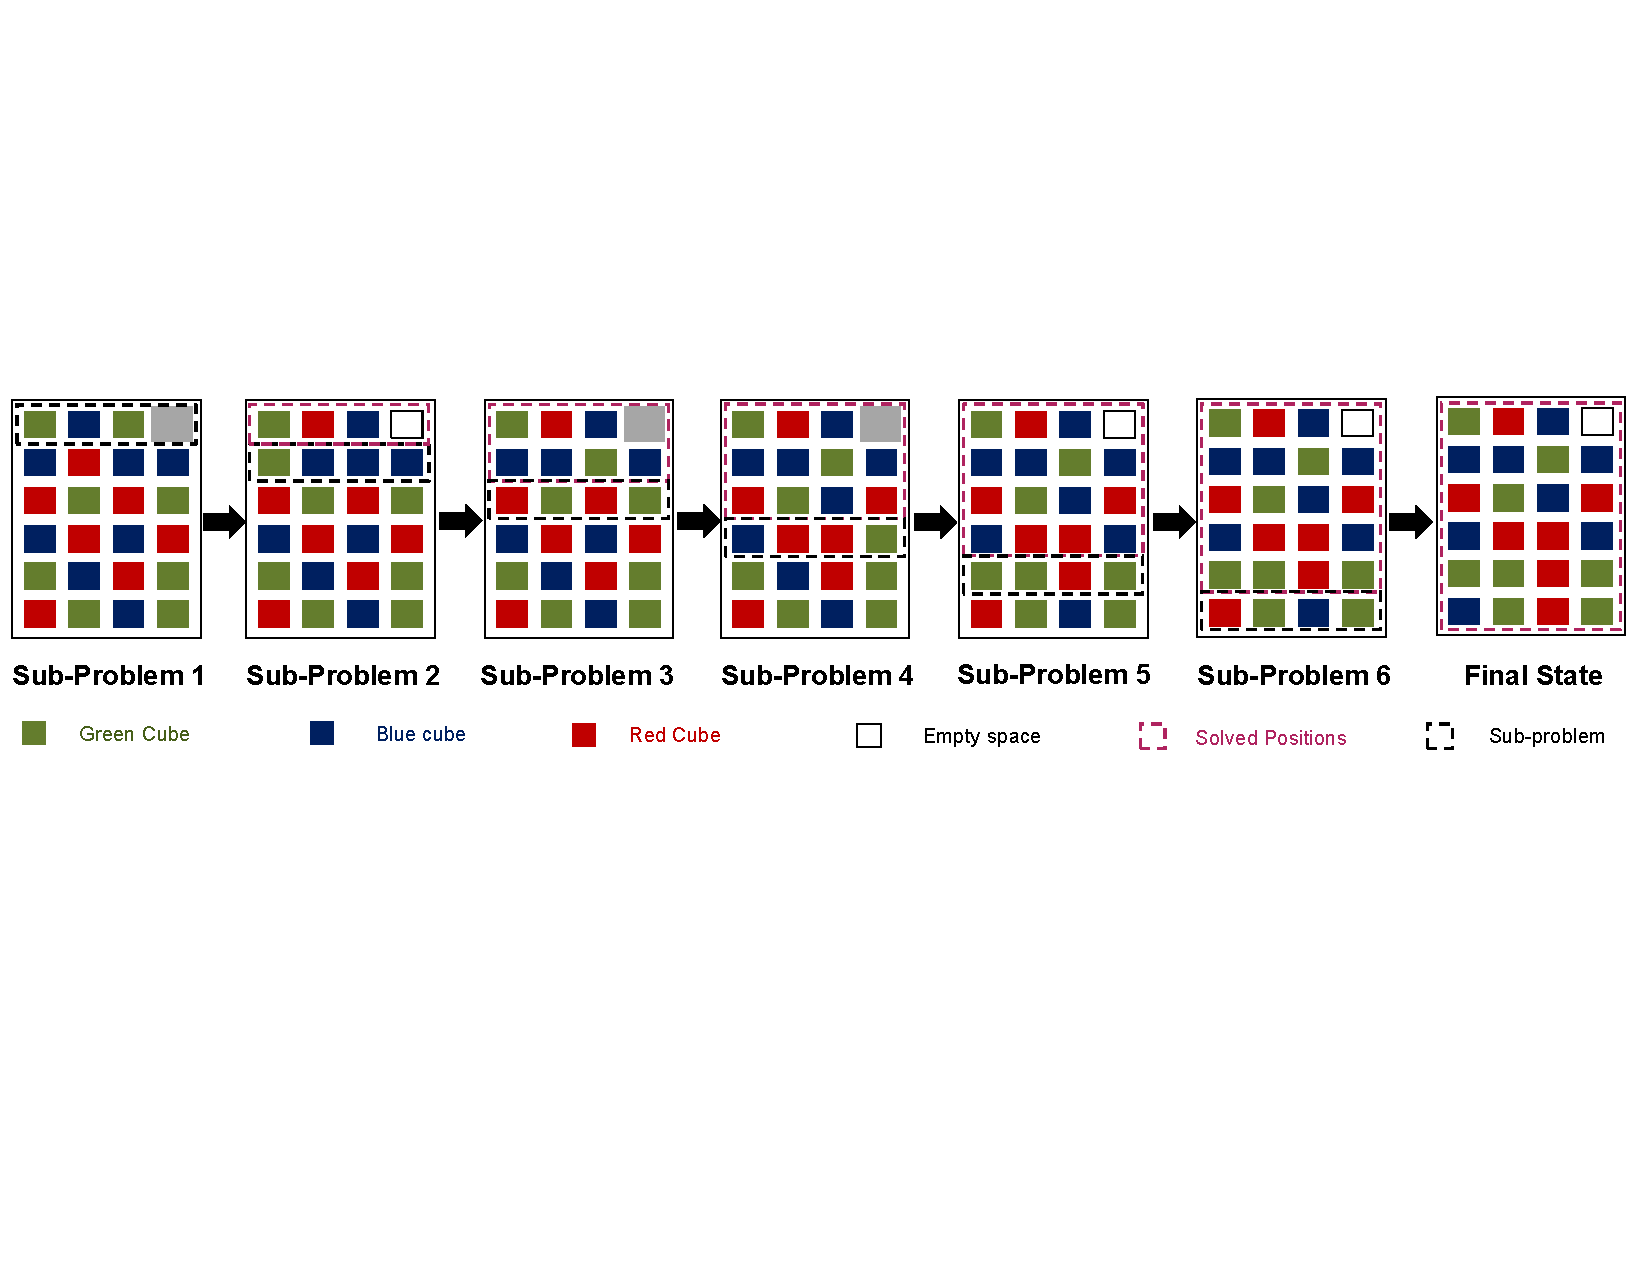
\includegraphics[width=\textwidth]{cropped_divide-conquer.pdf}
	\vspace{-0.1cm}
	\caption{Example illustrating the divide and conquer methodology for reducing solving time}
	\label{fig:divide}
\end{figure*}
\subsection{The Design Methodology of Industrial Gantry System}
The intelligent machine structure consists of a high-level planner to orchestrate the operations in low-level controller. The high-level planner renders autonomy to the system with an integrated motion and task planner. The algorithms of low-level controller lie in the realization and execution of motion profiles as per the instructions received from the high-level planner. The low-level controller is based on a technological controller (S7-1500T) which controls the modular servo drive system (SINAMICS S120). Each servo of the drive system is coupled to a linear system for required linear motion of Gantry Robot. We illustrated the relationship between the hardware and software components in Fig \ref{fig:asr4_}. 
Three servo-controller and linear motion systems are coupled to each other which enables the end-effector's motion in 3D- Cartesian Space. The Gantry Robots essentially contains three axes where each axis moves in the directions of x, y and z vectors (3D-Cartesian space). This implies that each point the end-effector of Gantry system traverses to computed x, y, and z coordinates. Additional two axes with rotational and servo-controlled gimbal mechanism allows for changing the orientation of the end-effector as shown in Fig \ref{fig:asr4_}. Moreover, the proposed system structure permits the control of 6-dof which the end-effector of the gantry system would perform in complex curvilinear paths or spline trajectories without an issue. In the current design, each point in space can be defined by x, y, z, ${\alpha}$ and ${\beta}$, where x, y, and z are linear distances while ${\alpha}$ and ${\beta}$ are the orientations.

\begin{figure*}[t]\vspace*{4pt}
\center
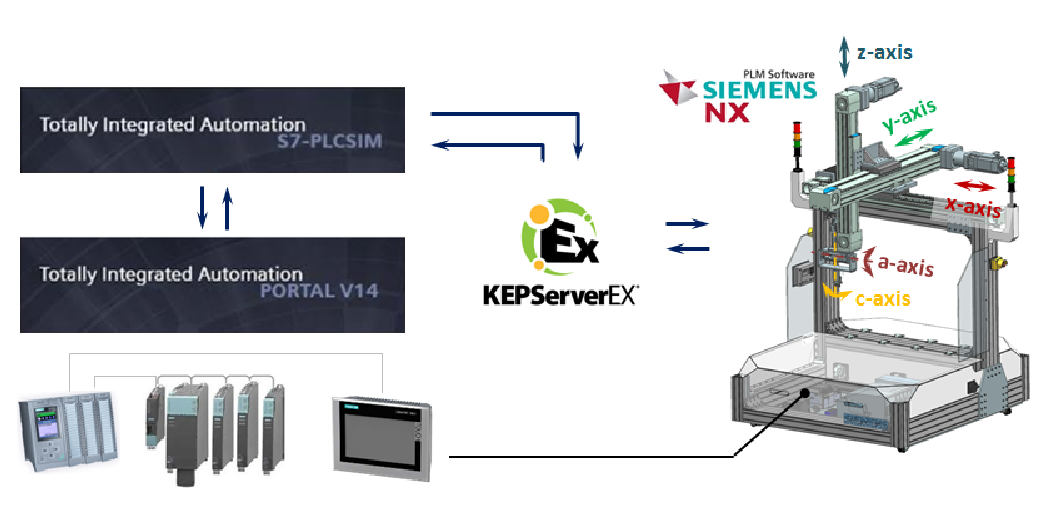
\includegraphics[width=0.7\textwidth]{asr4_}
\caption{The simulation and virtual commissioning architecture of intelligent machine tool (Gantry System)}
\label{fig:asr4_}
\end{figure*}

The low-level controller executes the synchronized linear and non-linear motion of multiple axes (servos) which Gantry Robot has 6-degrees of freedom. Such functionality utilizes e-CAM Technology in TIA Portal V 14.0 SP1, a proprietary SIEMENS development platform for the controllers such as S7 series. The controllers are designed with the capability to handle complex motion profile for synchronized multi-axes motion in real-time. The developed motion control library has a multi-segmented interpolation with a cyclic buffer which bolsters PLC controller for executing complex motion profiles in the run-time from high-level planners. We tested the motion control library up to thousand points -at once- in TIA Portal PLCSIM Advanced V2.0 which is also a proprietary SIEMENS software package. Due to the cyclic buffer the program can increase the total number of points without having any internal memory problems. PLCSIM Advanced emulates the technological functionality of a Siemens controller (e.g., S7-1500T series)\cite{plc_sim_adv} for striving virtual commissioning of cyber-physical system. Thus, PLCSIM Advanced and TIA Portal also assist the control engineer to tune and evaluate the actions (e.g., position, velocity profiles, acceleration and jerk limits, etc.) for the corresponding axis of cyber-physical systems. At the end, we generated a digital twin of the system and simulated the behaviors in Siemens NX Mechatronics Concept Designer (MCD). MCD simulates the systems under the given physics-based conditions with the control signals of real -or simulated- hardware.%{\newline}

KEPServerEX facilitates the connectivity between PLCSIM Advanced and NX due to the difference of the OPC protocols. TIA portal and PLCSIM Advanced are utilizing OPC UA whereas Siemens NX is OPC DA. KEPServerEX bridges between PLCSIM Advanced and NX and allows to share information while avoiding the discrepancies of OPC protocols. TIA Portal computes the necessary control actions. PLCSIM Advanced emulates the reaction of the TIA Portal's computations and maps computed parameters to Process Output Image of the controller. We setup KEPServerEX to use this mapping and pass the information to NX MCD which utilizes the incoming data and showcase the motion of Gantry Robot under physical constraints such as inertia, friction, and damping.

\section{Results}
For the described 2X2 toy example, our solver generated the safe and feasible solution in less than a second. As the grid size grows, one can observe that the solution time increases exponentially due to the size of the exploration space for the solver -the Boolean Satisfiability. Therefore, we reduced solving time by utilizing a receding-horizon-based divide and conquer approach, and divide the $A\times B$ grid into sub-problems, where the aim is to move $P$ cubes into their correct position, where $1<P\leq B$. %Each of these sub-problems consists of moving $P$ cubes into their correct position. 
For example, consider the $6\times 4$ grid, with 23 cubes and one empty buffer space. If we choose $P=4$, we can divide this problem into 6 sub problems. In the first sub problem, the aim is to get the positions 0 to 3 mapped to their correct cubes. Now, once this sub-problem is solved, positions 0 to 3 are solved, while positions 4 to 23 are unsolved. So in the next iteration, we solve to get the positions 4 to 7 solved. In doing so we consider only the positions between 4 and 23, and leave the cubes in positions 0 to 3 untouched (as they are already in place). Similarly, each sub-problem tries to move $P$ cubes into place without touching the cubes which have already been solved. However, to ensure that the solver does not get stuck, we also need to ensure that each sub-problem has an empty space (buffer) to enable cubes to be moved into their current position. Therefore, TL formulation in NUSMV-compatible description ensures that the empty space is always a part of the sub-problem being solved. Figure \ref{fig:divide}, shows an example 6X4 problem, which is solved using our proposed divide and conquer technique. 
When $P$ is sufficiently small, we can easily show that our technique, can enable the problem to be solved in linear time, i.e, if $P=B$, then the solution time is $O(A)$. This is because, we can show that to bring $P$ blocks into place, we need at most 2P steps, i.e., assuming all $P$ blocks are placed incorrectly, we need to move each incorrect cube to the buffer, and switch in the correct cube. Thus, for a given sub-problem of size $P$, the solving time can be upper bounded by a constant time term.

\begin{figure}[t]
	\centering
	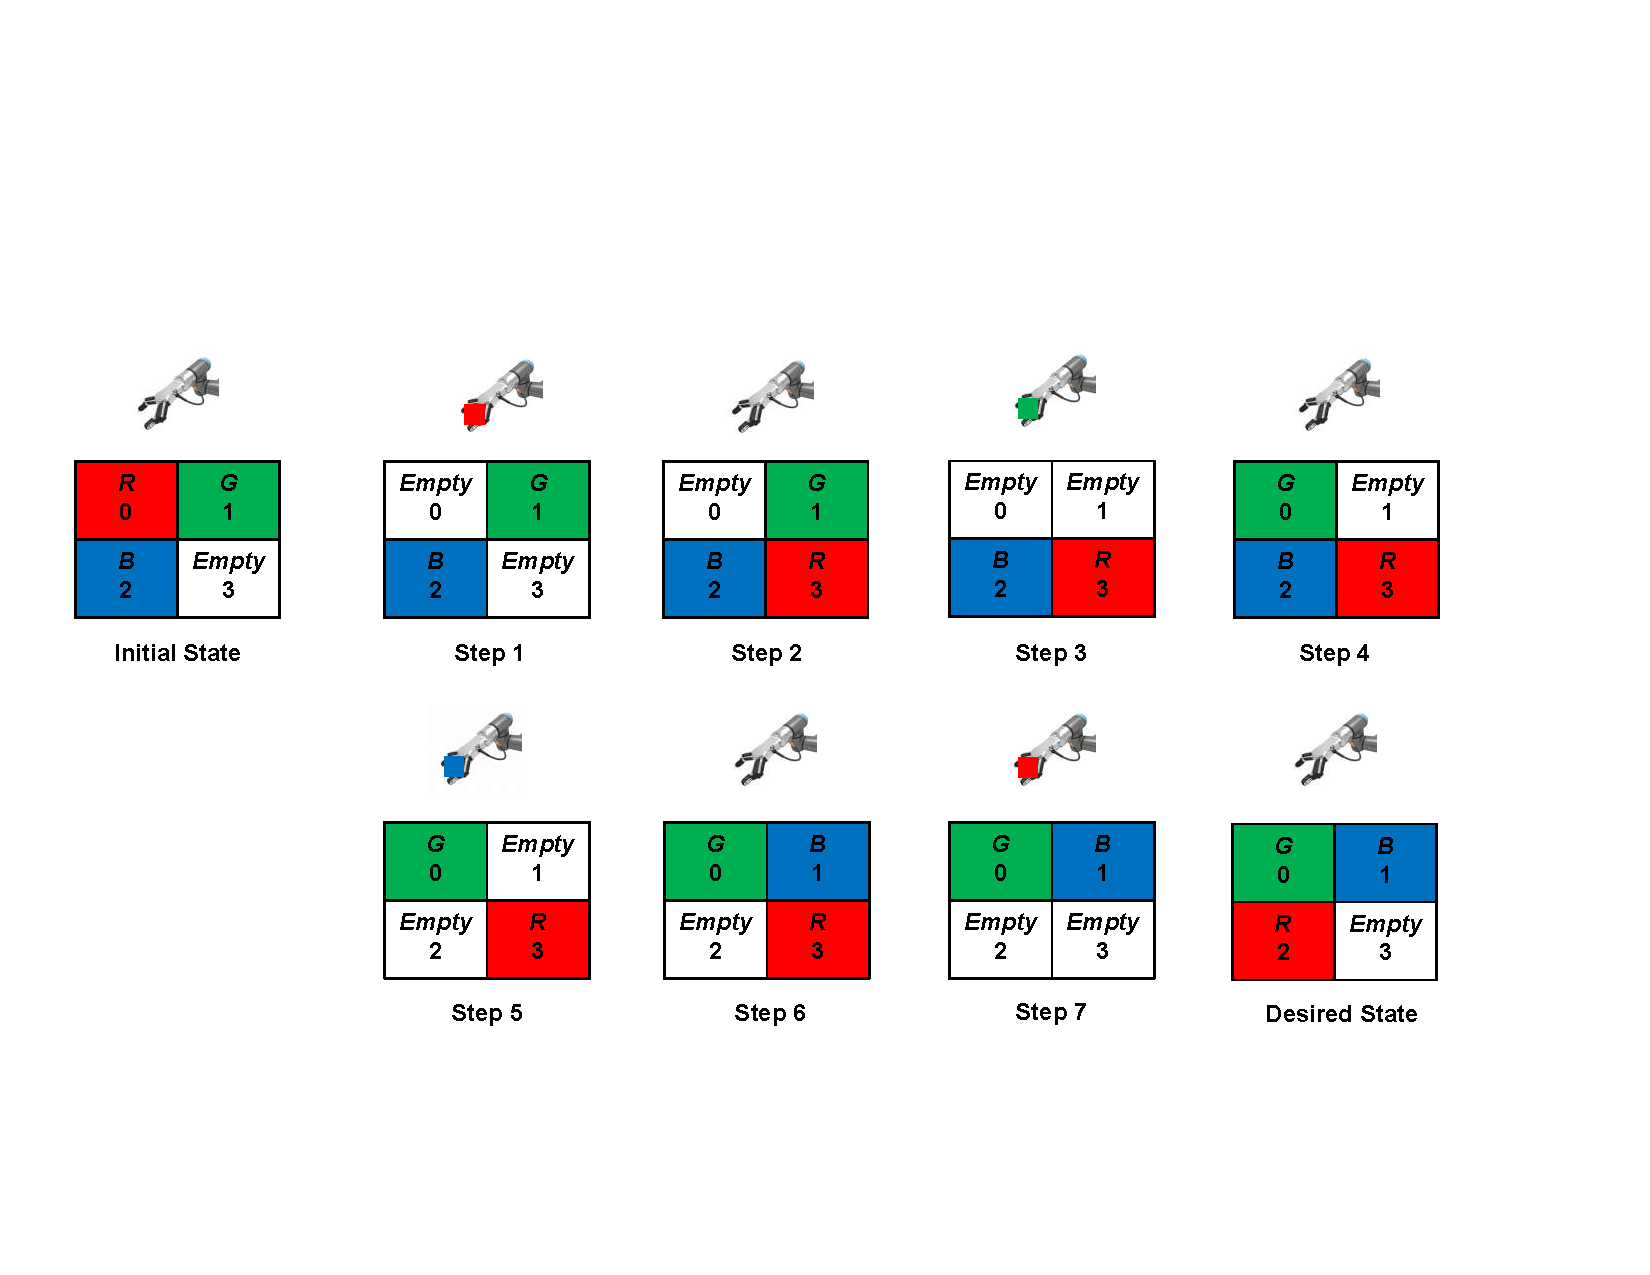
\includegraphics[width=\columnwidth]{planning_diagram.pdf} % Example image
	\vspace{-0.1cm}
	\caption{Example illustrating an feasible solution generated using our NuSMV-based solver package for a simple 2X2 problem. Each block in the grid highlights the color of the cube in the block, and its position. The gripper illustration highlights the cube in the gripper.}
	\label{fig:example}
\end{figure}

We tested number of cubes with a certain colors (e.g., y, g, b, r, an empty) 
in the proposed framework as well as standard NuSMV solver for benchmarking. 
We compared the speed and number of solution speed and number of solution steps 
on a S7-1518 TCPU. The solution reflects the scalability of our proposed framework 
in real-time system. 

\begin{table}[b]
\centering
\caption{Solving Time: Standard NuSMV vs. Proposed Framework}
\label{my-label}
\begin{tabular}{|l|l|l|}
\hline
           & \multicolumn{2}{c|}{Solution Time {[}sec{]}} \\
           \hline
\#of cubes & Standard NuSMV       & Proposed Framework   \\
\hline
4          & 0.4                  & 0.1                  \\
\hline
8          & 30                   & 0.2                  \\
\hline
16         & 100                  & 0.4                  \\
\hline
24         & 480                  & 0.8                  \\
\hline
100        & 3600                 & 3.1                 \\
\hline
\end{tabular}
\end{table}

\section{Conclusion and Further Work}
Emerging technologies (e.g. Industry 4.0) will shift the paradigm in Advanced Manufacturing, where manufacturers try to adapt these technologies on factory floor and enabling Smart Manufacturing Systems. These adaptation will bring new safety issues which would be hard to encode in runtime intelligence of cyber-physical system. Therefore, we introduced TL-based autonomy for smart manufacturing systems to have an intuitive and easy to use framework for hybrid -continuous and discrete- systems.

We showcased an industry-inspired implementation via simulation as well as real Gantry Robot. The Gantry Robot and its skill (assembly) represents an abstraction which can be changed into different planning aspects for the manufacturing process flow. At the end of the day, our method will assist to the system integrators or plant workers for enabling safe autonomy of cyber-physical systems. We see the proposed framework as a generic tool to employ the increasing need in different part of the factories.

Robust and interoperable methods with standardized interface protocols are imperative to have autonomous and smart manufacturing for having a broader impact in different industries. The application of proposed TL-based autonomy framework under a standardized interface protocol (e.g., MTConnect) would bolster a wider use of our framework for different machine-tools (e.g., Mazak, DMC, Mori Seiki, etc.) as well as controllers. Lastly, controller synthesis for hybrid systems that satisfy temporal specifications expressing various system properties under uncertainties is more realistic for manufacturing operations. Instead of utilizing learning based solutions to cope with the uncertainties, probability infused TL would be an alternative solution. Therefore, we plan to add probabilistic operators in our Temporal Logic (PrTL) framework which will incorporate stochastic mathematical specifications to enforce safety under uncertainties. Lastly, the proposed method facilitates a safe and feasible solution rather than optimal, we leave the optimal form of the LTL solution for our future work.

\section*{Acknowledgements}

The authors would like to thank to Lingyun Wang, Research Group Head of the Product Runtime System Group and Kurt Bettenhausen, Senior Vice President of Siemens Corporation Corporate Technology for providing the funding under Autonomous System Revolution (ASR) Project.

%% References
%%
%% Following citation commands can be used in the body text:
%% Usage of \cite is as follows:
%%   \cite{key}         ==>>  [#]
%%   \cite[chap. 2]{key} ==>> [#, chap. 2]
%%

%The citation must be used in following style: \cite{article-minimal} \cite{article-full} \cite{article-crossref} \cite{whole-journal}.
%% References with BibTeX database:

%\bibliography{xampl}
%\bibliographystyle{model1a-num-names}


%% Authors are advised to use a BibTeX database file for their reference list.
%% The provided style file elsarticle-num.bst formats references in the required Procedia style

%% For references without a BibTeX database:
\vspace*{-3pt}
\begin{thebibliography}{}

%% \bibitem must have the following form:
%%   \bibitem{key}...

%% PLEASE USE CHICAGO FORMAT
\vspace*{-3pt}
\bibitem{digit_twin}
Rosen, Roland, Georg von Wichert, George Lo, and Kurt D. Bettenhausen. \quotes{About the importance of autonomy and digital twins for the future of manufacturing.} \emph{IFAC-PapersOnLine} 48, no. 3 (2015): 567-572.
\bibitem{smart_man}
Ramakrishna, Seeram, Tham Chen Khong, and Teo Kie Leong. \quotes{Smart Manufacturing.} \emph{Procedia Manufacturing} 12 (2017): 128-131.
\bibitem{cyber_sec}
Vincent, Hannah, Lee Wells, Pablo Tarazaga, and Jaime Camelio. \quotes{Trojan detection and side-channel analyses for cyber-security in cyber-physical manufacturing systems.} \emph{Procedia Manufacturing} 1 (2015): 77-85.
\bibitem{hotcloud}
Sandeep D'souza and Raj Rajkumar, \quotes{Time-based Coordination in Geo-Distributed Cyber-Physical Systems}, in Proc. of \emph{USENIX Workshop on Hot Topics on Cloud Computing}, 2017
\bibitem{cloud_manuf}
Wang, Peng, Robert X. Gao, and Zhaoyan Fan. \quotes{Cloud computing for cloud manufacturing: benefits and limitations.} \emph{Journal of Manufacturing Science and Engineering} 137, no. 4 (2015): 040901.
\bibitem{ros_item}
Quigley, Morgan, Ken Conley, Brian Gerkey, Josh Faust, Tully Foote, Jeremy Leibs, Rob Wheeler, and Andrew Y. Ng. \quotes{ROS: an open-source Robot Operating System.} \emph{In ICRA workshop on open source software}, vol. 3, no. 3.2, p. 5. 2009.
\bibitem{nusmv2}
Cimatti, Alessandro, Edmund Clarke, Enrico Giunchiglia, Fausto Giunchiglia, Marco Pistore, Marco Roveri, Roberto Sebastiani, and Armando Tacchella. \quotes{Nusmv 2: An opensource tool for symbolic model checking.} \emph{In International Conference on Computer Aided Verification}, pp. 359-364. Springer, Berlin, Heidelberg, 2002.
\bibitem{ltl_phm}
Heddy, Gerald, Umer Huzaifa, Peter Beling, Yacov Haimes, Jeremy Marvel, Brian Weiss, and Amy LaViers. \quotes{Linear Temporal Logic (LTL) Based Monitoring of Smart Manufacturing Systems.} (2015): 10.
\bibitem{ltl_mod}
Mazzolini, Mauro, Alessandro Brusaferri, and Emanuele Carpanzano. \quotes{Model-checking based verification approach for advanced industrial automation solutions.} \emph{In Emerging Technologies and Factory Automation (ETFA), 2010 IEEE Conference} on, pp. 1-8. IEEE, 2010.
\bibitem{ltl_plc}
Ljungkrantz, Oscar, Knut Åkesson, Martin Fabian, and Chengyin Yuan. \quotes{A formal specification language for PLC-based control logic.} \emph{In Industrial Informatics (INDIN), 2010 8th IEEE International Conference} on, pp. 1067-1072. IEEE, 2010.
\bibitem{ltl_formal}
Dokhanchi, Adel, Bardh Hoxha, and Georgios Fainekos. \quotes{Formal requirement debugging for testing and verification of cyber-physical systems.} \emph{arXiv preprint} arXiv:1607.02549 (2016).
\bibitem{ltl_control}
Belta, Calin, Antonio Bicchi, Magnus Egerstedt, Emilio Frazzoli, Eric Klavins, and George J. Pappas. \quotes{Symbolic planning and control of robot motion [grand challenges of robotics].} \emph{IEEE Robotics and Automation Magazine} 14, no. 1 (2007): 61-70.
\bibitem{LTL} 
Li Tan, Oleg Sokolsky, and Insup Lee, \quotes{Specification-Based Testing with Linear Temporal Logic}, in Proc. of \emph{IEEE International Conference on Information Reuse and Integration}, 2004
\bibitem{ltl-planning}
Marius Kloetzer and Cristian Mahulea, \quotes{LTL-Based Planning in Environments with Probabilistic Observations}, in \emph{IEEE Transactions on Automation Science and Engineering}, Vol. 12, No. 4, October 2015
\bibitem{model-book}
Baier, Christel, Joost-Pieter Katoen, and Kim Guldstrand Larsen. \quotes{Principles of model checking.} \emph{MIT press}, 2008.
\bibitem{NIST}
The  National  Institute  of  Standards  and  Technology  (NIST), \quotes{Safety of human-robot systems in fixed workcell environments.},http://www.nist.gov, 2014.
\bibitem{ISO-15066}
International  Organization  for  Standardization, \quotes{ISO/DTS  15066  Robots  and  robotic  devices  –  Safety  requirements  for  industrial  robots  –  Collaborative  operation.}, http://www.iso.org, 2014.
\bibitem{ISO-10218}
International  Organization  for  Standardization, \quotes{ISO  10218-1:2011  Robots  and  robotic  devices  –  Safety  requirements for industrial robots – Part 1: Robots.}, http://www.iso.org, 2011.
\bibitem{low_level_cont}
Ferraguti, Federica, Chiara Talignani Landi, Cristian Secchi, Cesare Fantuzzi, Marco Nolli, and Manuel Pesamosca. \quotes{Walk-through Programming for Industrial Applications.} \emph{Procedia Manufacturing} 11 (2017): 31-38.
\bibitem{Strunk} W. Strunk Jr., E.B. White, \quotes{The Elements of Style}, third ed., Macmillan, New York, 1979.
\bibitem{Mettam} G.R. Mettam, L.B. Adams, in: B.S. Jones, R.Z. Smith (Eds.), \quotes{Introduction to the Electronic Age}, \emph{E-Publishing Inc.}, New York, 1999, pp. 281--304.
\bibitem{plc_sim_adv}
Berger, Hans. \quotes{Automating with SIMATIC: controllers, software, programming, data.} \emph{John Wiley and Sons}, 2012.
 \end{thebibliography}
\end{document}

\clearpage

%%%% This page is for instructions only, once the article is finalize please omit the below text before creating the final PDF
\normalMode

\section*{Instructions to Authors for LaTeX template:}

\section{ZIP mode for LaTeX template:}

The zip package is created as per the guide lines present on the URL http://www.elsevier.com/author-schemas/ preparing-crc-journal-articles-with-latex for creating the LaTeX zip file of Procedia LaTeX template.  The zip generally contains the following files:
\begin{Itemize}[]\leftskip-17.7pt\labelsep3.3pt
\item ecrc.sty
\item  elsarticle.cls
\item elsdoc.pdf
\item .bst file
\item Manuscript templates for use with these bibliographic styles
\item  Generic and journal specific logos, etc.
\end{Itemize}

The LaTeX package is the main LaTeX template. All LaTeX support files are required for LaTeX pdf generation from the LaTeX template package.

{\bf Reference style .bst file used for collaboration support:} In the LaTeX template packages of all Procedia titles a new ``.bst'' file is used which supports collaborations downloaded from the path http://www.elsevier.com/author-schemas/the-elsarticle-latex-document-class

\section{Reference styles used in  Procedia master templates:}
\makeatletter
\@namedef{tabular*}#1{\normalsize%
 \setlength\dimen@{#1}%
   \edef\@halignto{to\the\dimen@}\@tabular}
\makeatother
%\let\footnotesize\normalsize
\hspace*{-10pt}\begin{tabular*}{\hsize}{@{}ll@{}}
{\bf Title}&{\bf Reference style} \\[6pt]
AASPRO  & 2 Harvard\\
AASRI Procedia  & 3 Vancouver Numbered\\
APCBEE Procedia  & 3 Vancouver Numbered\\
EGYPRO  & 3 Vancouver Numbered\\
FINE    & 2 Harvard\\
IERI Procedia  & 3 Vancouver Numbered\\
MATPR  & 1a Numbered without article titles\\
MSPRO  & 2 Harvard\\
PHPRO  & 2 Harvard\\
PIUTAM  & 3a Embellished Vancouver \\
Procedia CIRP  & 3 Vancouver Numbered\\
PROCHE  & 3a Embellished Vancouver \\
PROCS  & 3a Embellished Vancouver \\
PROENG  & 1 Numbered\\
PROENV  & 3a Embellished Vancouver \\
PROEPS  & 3a Embellished Vancouver \\
PROFOO    & 3a Embellished Vancouver \\
PROMFG  & 1a Numbered without article titles\\
PROTCY  & 3 Vancouver Numbered\\
PROVAC  & 3a Embellished Vancouver \\
SBSPRO  & 5 APA\\
SEPRO  & 3a Embellished Vancouver \\
AQPRO & 2 Harvard\\
UMKPRO & 5 APA\\
\end{tabular*}


\end{document}

%%
%% End of file `procs-template.tex'.
